\begin{extask}{4-3}
  \subsection*{課題内容}
  \texttt{socket\_dns\_test.py}が生成したDNS問い合わせパケットの内容を確認し，DNSの規定に沿っているかを調べる．

  \subsection*{実験方法}
  \begin{enumerate}
    \item 4-2で取得したpcapをWiresharkで開き，DNS Queryパケットを選択する．
    \item DNSヘッダとQuestionセクションを展開し，ID，フラグ，質問数，問い合わせ名，問い合わせ型，クラスを確認する．
    \item 指導書で指定されたDNS形式・RFCの記述と照合する．
  \end{enumerate}

  \subsection*{結果}
  DNS問い合わせパケットの画面を図\ref{fig:dns_format}に示す．
  \begin{figure}[H]
    \centering
    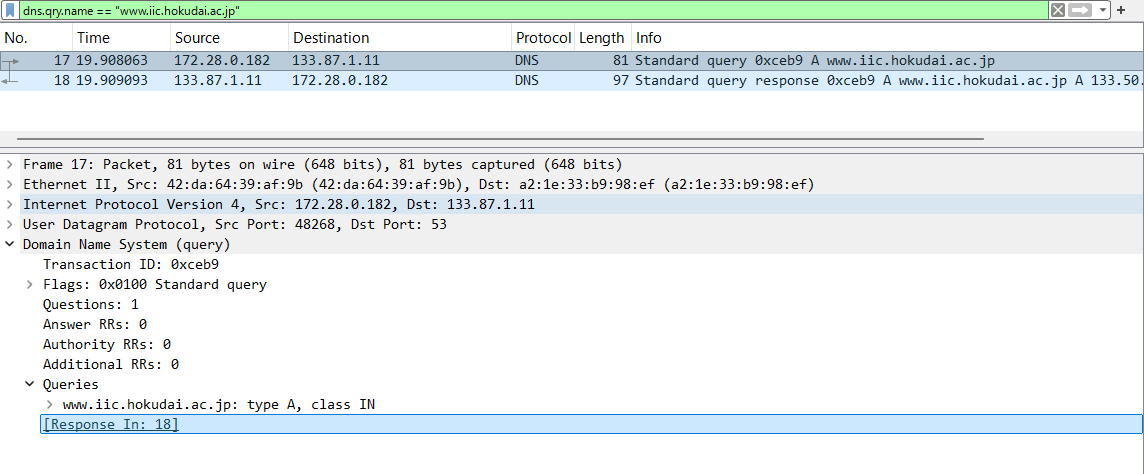
\includegraphics[width=0.98\columnwidth]{fig/wireshark_day4_3_dns_format.png}
    \par\smallskip
    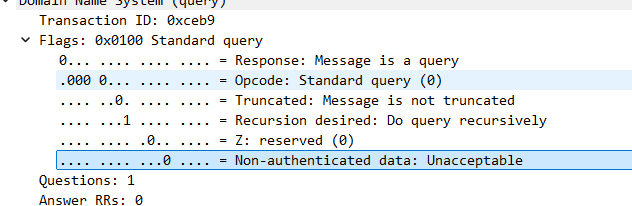
\includegraphics[width=0.72\columnwidth]{fig/wireshark_day4_3_dns_flags.png}
    \par\smallskip
    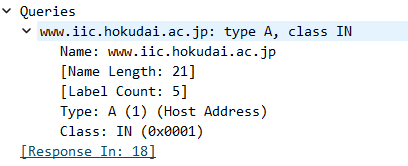
\includegraphics[width=0.72\columnwidth]{fig/wireshark_day4_3_dns_question.png}
    \caption{DNS問い合わせパケットの構造}\label{fig:dns_format}
  \end{figure}

  Wiresharkで確認したTransaction IDは\texttt{0xceb9}，Flagsは\texttt{0x0100}，Questionsは1であり，Answer/Authority/Additional RRsはいずれも0であった．Flagsの内訳は，QR=0（問い合わせ），Opcode=0（標準問い合わせ），TC=0（切り詰めなし），RD=1（再帰問い合わせ希望），予約ビット=0，AD=0であった．ADビットを問い合わせでクリアする形式はRFC 4035 §4.6にも沿っている．QuestionはQNAME=\texttt{www.iic.hokudai.ac.jp}，QTYPE=A（1），QCLASS=IN（\texttt{0x0001}）である．DNSヘッダおよび質問部の形式を定めるRFC 1035 §4.1.1–4.1.2と照合し，確認した値は標準問い合わせの形式に沿っていることを確認した．
\end{extask}
